\documentclass[aspectratio=43]{beamer}%[handout]
\mode<handout>{
\usepackage{pgfpages}
\pgfpagesuselayout{4 on 1}[letterpaper,border shrink=5mm, landscape]
}
\usepackage[T1]{fontenc}
\usepackage[utf8]{inputenc}
\usepackage[spanish]{babel}
\usepackage{beamerthemeshadow,beamerthemesplit,cite,cancel,lmodern,eso-pic,fancyvrb,textcomp,lmodern,url,times,booktabs,amssymb,amsmath,ragged2e,float,subfig,xspace,epic,eepic,multicol,multirow,colortbl,color,graphicx,url}
\usepackage[normalem]{ulem} %tachar texto con \sout{}
\usepackage{listings} %CODIGOs
\usepackage[sfdefault]{roboto}
\setcounter{tocdepth}{3}
\usepackage[figurename=]{caption}
%Colores Ulagos
\definecolor{gray97}{gray}{.97}
\definecolor{gray75}{gray}{.75}
\definecolor{gray45}{gray}{.45}
\definecolor{listinggray}{gray}{0.9}
\definecolor{lbcolor}{rgb}{0.9,0.9,0.9}
%Colores Ulagos
\definecolor{amarillo}{RGB}{255,182,18}
\definecolor{verde}{RGB}{52,178,51}
\definecolor{rojo}{RGB}{237,41,57}
\definecolor{azulu}{RGB}{19,15,204}
\definecolor{azul}{RGB}{1,110,185}
\definecolor{negro}{RGB}{35,31,32}
\definecolor{naranjo}{RGB}{251,79,20}
\newcommand\rojo[1]{\textcolor[RGB]{237,41,57}{#1}}
\newcommand\gris[1]{\textcolor[gray]{.65}{#1}}
\newcommand\azul[1]{\textcolor[RGB]{19,15,204}{#1}}
\newcommand\verde[1]{\textcolor[RGB]{5,101,99}{#1}}
\newcommand\naranjo[1]{\textcolor[RGB]{251,79,20}{#1}}

%%%%%%%%%%%%%%%%%%%%%%%%%
%% Tikz
%%%%%%%%%%%%%%%%%%%%%%%%%
\usepackage{tikz}
\usetikzlibrary{trees}
\usetikzlibrary{snakes}
\usetikzlibrary{arrows}
\usetikzlibrary{shapes}
\usetikzlibrary{backgrounds}
\usetikzlibrary{patterns}
\usetikzlibrary{fit}
\usetikzlibrary{positioning} % LATEX and plain TEX
%%%%%%%%%%%%%%%%%%%%%%%%%%

%%%%%%%%%%%%%%%%%%%%%TEMA
\mode<presentation>
\usetheme{CambridgeUS}
\usecolortheme[named=azul]{structure}
\useinnertheme{rectangles}    
\useoutertheme{infolines} 
               
\setbeamercovered{transparent}

\setbeamerfont{block title}{size={}}
\setbeamerfont{title}{shape=\scshape}
\setbeamerfont{frametitle}{shape=\scshape}
\setbeamerfont{author}{shape=\scshape}
\setbeamerfont{institute}{shape=\scshape}
\setbeamerfont{block title}{shape=\scshape}

\setbeamertemplate{blocks}[rounded][shadow=true]
\setbeamertemplate{itemize items}[default]
\setbeamertemplate{enumerate items}[circle]
\setbeamertemplate{description item}[align left]
\setbeamertemplate{blocks}[rounded][shadow=true]
\setbeamertemplate{title page}[default][colsep=-4bp,rounded=false,shadow=false]
%\setbeamertemplate{frametitle continuation}

\setbeamercolor*{palette primary}{use=structure,fg=azul,bg=listinggray}
\setbeamercolor*{palette secondary}{use=structure,fg=azul,bg=gray97}
\setbeamercolor*{palette tertiary}{use=structure,fg=gray97,bg=azul}
\setbeamercolor*{palette sidebar primary}{use=structure,fg=azul}
\setbeamercolor*{palette sidebar tertiary}{use=structure,fg=azul}
\setbeamercolor*{title}{use=structure,fg=white}
\setbeamercolor*{author}{use=structure,fg=white}
\setbeamercolor*{institute}{use=structure,fg=white}
\setbeamercolor{frametitle right}{bg=azul!50!white}
\setbeamercolor{structure}{fg=azul}
\setbeamercolor{block title}{use=structure,fg=white,bg=amarillo}
\setbeamercolor{block body}{use=structure,fg=negro,bg=amarillo!20!white}
\setbeamercolor{block title example}{use=structure,fg=white,bg=verde!80!black}
\setbeamercolor{block body example}{use=structure,fg=negro,bg=verde!20!white}
\setbeamercolor{block title alerted}{use=structure,fg=white,bg=rojo!90!negro}
\setbeamercolor{block body alerted}{use=structure,fg=negro,bg=rojo!20!white}
%%%%%%%%%%%%%%%%%%%%%FIN TEMA

%lstlisting %%%%%CODIGOS
\lstset{tabsize=4,language=C,basicstyle=\small,upquote=true,aboveskip={1.5\baselineskip},columns=fixed,showstringspaces=false, extendedchars=true,breaklines=true, prebreak = \raisebox{0ex}[0ex][0ex]{\color{gray75}{\ensuremath{\hookleftarrow}}},showtabs=false,showspaces=false,showstringspaces=false,identifierstyle=\ttfamily,keywordstyle=\color[rgb]{0,0,1}, commentstyle=\color[rgb]{0.133,0.545,0.133}, stringstyle=\color[rgb]{0.627,0.126,0.941}} 
  
%%%%%%%%%%%%%%PORTADA
\title[Introducción a \LaTeX{}]{\textbf{\huge{Introducción a \LaTeX{}}}\vspace{-0.3cm}}
\subtitle{Formación General\vspace{-0.7cm}}
\author[Juan José Ramírez Lama]{\small{\textbf{Juan José Ramírez Lama} \\  \texttt{juan.ramirez@ulagos.cl}}\vspace{-0.2cm}}
\institute[ULA]{\small{\textbf{Departamento de Ciencias Exactas}\\Ingeniería Civil en Informática}\vspace{-0.5cm}}
\date[\today]{}
%%%%%%%%%%%%%FIN PORTADA

\begin{document}
\setbeamertemplate{background}{
\includegraphics[height=9.2cm,width=12.8cm]{fondoula43}}%4:3
%\setbeamertemplate{background}{\centering\includegraphics[height=8.6cm,width=16.1cm]{fondoula169}}%16:9


%Pagina de Portada
\begin {frame} [plain]
\vspace{5.25cm}
\titlepage
\end {frame}
\setbeamertemplate{background}{}
%%%%%%%%%%%%%%%%ÍNDICES
\section[Contenido]{}
\frame{
  \frametitle{\textbf{Contenido}}
\setcounter{tocdepth}{2}%1: solo titulo principal, 2: titulo y subtitulo, 3....
\scriptsize
\tableofcontents[]
}%Generacion de Indice por capitulo
\AtBeginSection[]{
\begin{frame}
\frametitle{\textbf{Contenido}}
\scriptsize
\tableofcontents[currentsection]
\end{frame}}

\AtBeginSubsection[]{
\begin{frame}
\frametitle{\textbf{Contenido}}  
\scriptsize
\tableofcontents[currentsection,currentsubsection]
\end{frame}
}
%%%%%%%%%%%%%%%%FIN ÍNDICES







%%%%%%%%%%%%%%%%%%%%%%%%%%%%%%%%%%%%%
%%%%%%%%%%%%%%%%%INICIO PRESENTACION

\section{Modelo Literario}
\begin{frame}[fragile]
\frametitle{\textbf{Modelo Literario}}
\justifying
 \begin{itemize}\justifying
  \item La programación literaria es un paradigma de programación propuesto por Donald Knuth como alternativa al popular paradigma de programación estructurada en la década de 1970.
  \item El paradigma de programación literaria, tal y como lo concibió Knuth, representa un movimiento disruptivo respecto a la escritura de programas en el orden y forma impuesto por el ordenador. En cambio permite a los programadores desarrollar sus programas en el orden fijado por la lógica y el flujo de sus pensamientos.
\end{itemize}
\end{frame}


\begin{frame}[fragile]
\frametitle{\textbf{Modelo Literario}}
\justifying
\begin{itemize}\justifying
  \item  Los programas literarios están escritos como una exposición lógica no interrumpida en un lenguaje humano, de forma similar al texto de un ensayo, en el cual se incluye el código fuente tradicional oculto tras macros. 
  \item Las herramientas de programación se encargan de separar el programa de forma que pueda ser compilado y ejecutado y la documentación del mismo programa. 
  \item Mientras que las primera generación de herramientas de programación literaria estaban centradas en un lenguaje de programación específico, las últimas son independientes de lenguaje y se sitúan por encima de los lenguajes de programación.
\end{itemize}


\end{frame}

\begin{frame}[fragile]
\frametitle{\textbf{Principales Lenguajes}}
\justifying
 \begin{itemize}\justifying
  \item \TeX{}
  \item TyX
  \item \LaTeX{}
\end{itemize}

\end{frame}


\begin{frame}[fragile]
\frametitle{\textbf{Ejemplo \LaTeX{}}}
\justifying
 \begin{block}{Código}
   \lstset{language=TEX,basicstyle=\small}
   \vspace{-0.8cm}
\begin{lstlisting}
\begin{displaymath}
C_L=\frac{(S_{22}-\Delta S_{11}^*)^*}{|S_{22}|^2=-|\Delta|^2}
\end{displaymath}
    
\[
R_S=\frac{\sqrt{1-g_s}\cdot (1-|S_{11}|^2)}{1-(1-g_s)\cdot|S_{11}|^2}
\]
\end{lstlisting}\vspace{-0.3cm}

\end{block}


\begin{exampleblock}{Resultado}
\begin{displaymath}
C_L=\frac{(S_{22}-\Delta S_{11}^*)^*}{|S_{22}|^2=-|\Delta|^2}
\end{displaymath}
    
\[
R_S=\frac{\sqrt{1-g_s}\cdot (1-|S_{11}|^2)}{1-(1-g_s)\cdot|S_{11}|^2}
\]

\end{exampleblock}

\end{frame}

\subsection{?`Por qué usar \LaTeX{}?}

\begin{frame}[fragile]
\frametitle{\textbf{?`Por qué usar \LaTeX{}?}}
\justifying
 \begin{itemize}\justifying
  \item Porque queremos publicar un artículo y nos envían una plantilla \LaTeX{}.
  \item Otras personas de nuestro grupo de trabajo (o investigación) lo usan, y queremos editar documentos de forma colaborativa.
  \item Para crear fácilmente documentos largos manteniendo el formato y calidad (tesis).
  \item Para publicar libros.
\end{itemize}
\end{frame}

\begin{frame}[fragile]
\frametitle{\textbf{?`Qué nos aporta \LaTeX{}?}}
\justifying
 \begin{itemize}\justifying
  \item Permite crear fácilmente documentos de alta calidad.
  \item Fácil escritura de matemáticas complejas.
  \item Sistema muy estable, portable y estándar.
  \item Posibilidad de dividir el documento en varios archivos.
  \item Creación de presentaciones de aspecto profesional.
\end{itemize}
\end{frame}

\subsection{?`Qué es \TeX{}?}
\begin{frame}[fragile]
\frametitle{\textbf{?`Qué es \TeX{}?}}
\justifying
 Programa tipográfico creado por Donald E. Knuth en 1982.
 \begin{center}
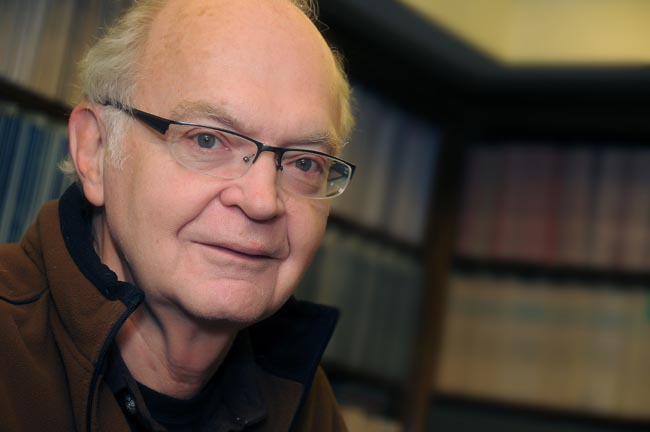
\includegraphics[width=10cm]{images/d_knuth_noticia}
\end{center}
\end{frame}

\begin{frame}[fragile]
\frametitle{\textbf{Donald E. Knuth}}
\justifying
 \begin{itemize}\justifying
  \item Experto en Ciencias de la Computación en el área de \textbf{Análisis de Algoritmos y Compiladores}.
  \item Autor de ``El Arte de Programar Computadoras''.
  \item Sentó las bases y dio nombre al análisis de algoritmos.
  \item Creador de \TeX{} y de la Programación Literaria.
  \item \azul{Premio Donald E. Knuth}: Otorgado a quienes realizan contribuciones destacadas sobre los fundamentos de Cs. de la Computación.
\end{itemize}

\end{frame}

\begin{frame}[fragile]
\frametitle{\textbf{?`Qué es \TeX{}?}}
\justifying
 \begin{itemize}\justifying
  \item Programa diseñado para publicar texto y fórmulas matemáticas con gran calidad tipográfica.
  \item Pretendía invertir la tendencia a una \textit{calidad tipográfica en declive} que afectaba a sus propios libros y artículos.
  \item Increíblemente estable: se considera libre de bugs.
  \item El número de versión converge a $\pi$, y es actualmente 3,14159265.
\end{itemize}
\[\pi= 3,14159265358979323846\]
\end{frame}

\subsection{?`Qué es \LaTeX{}?}
\begin{frame}[fragile]
\frametitle{\textbf{?`Qué es \LaTeX{}?}}
\justifying
Un paquete de macros para \TeX{} escrito por Leslie Lamport.
\begin{center}
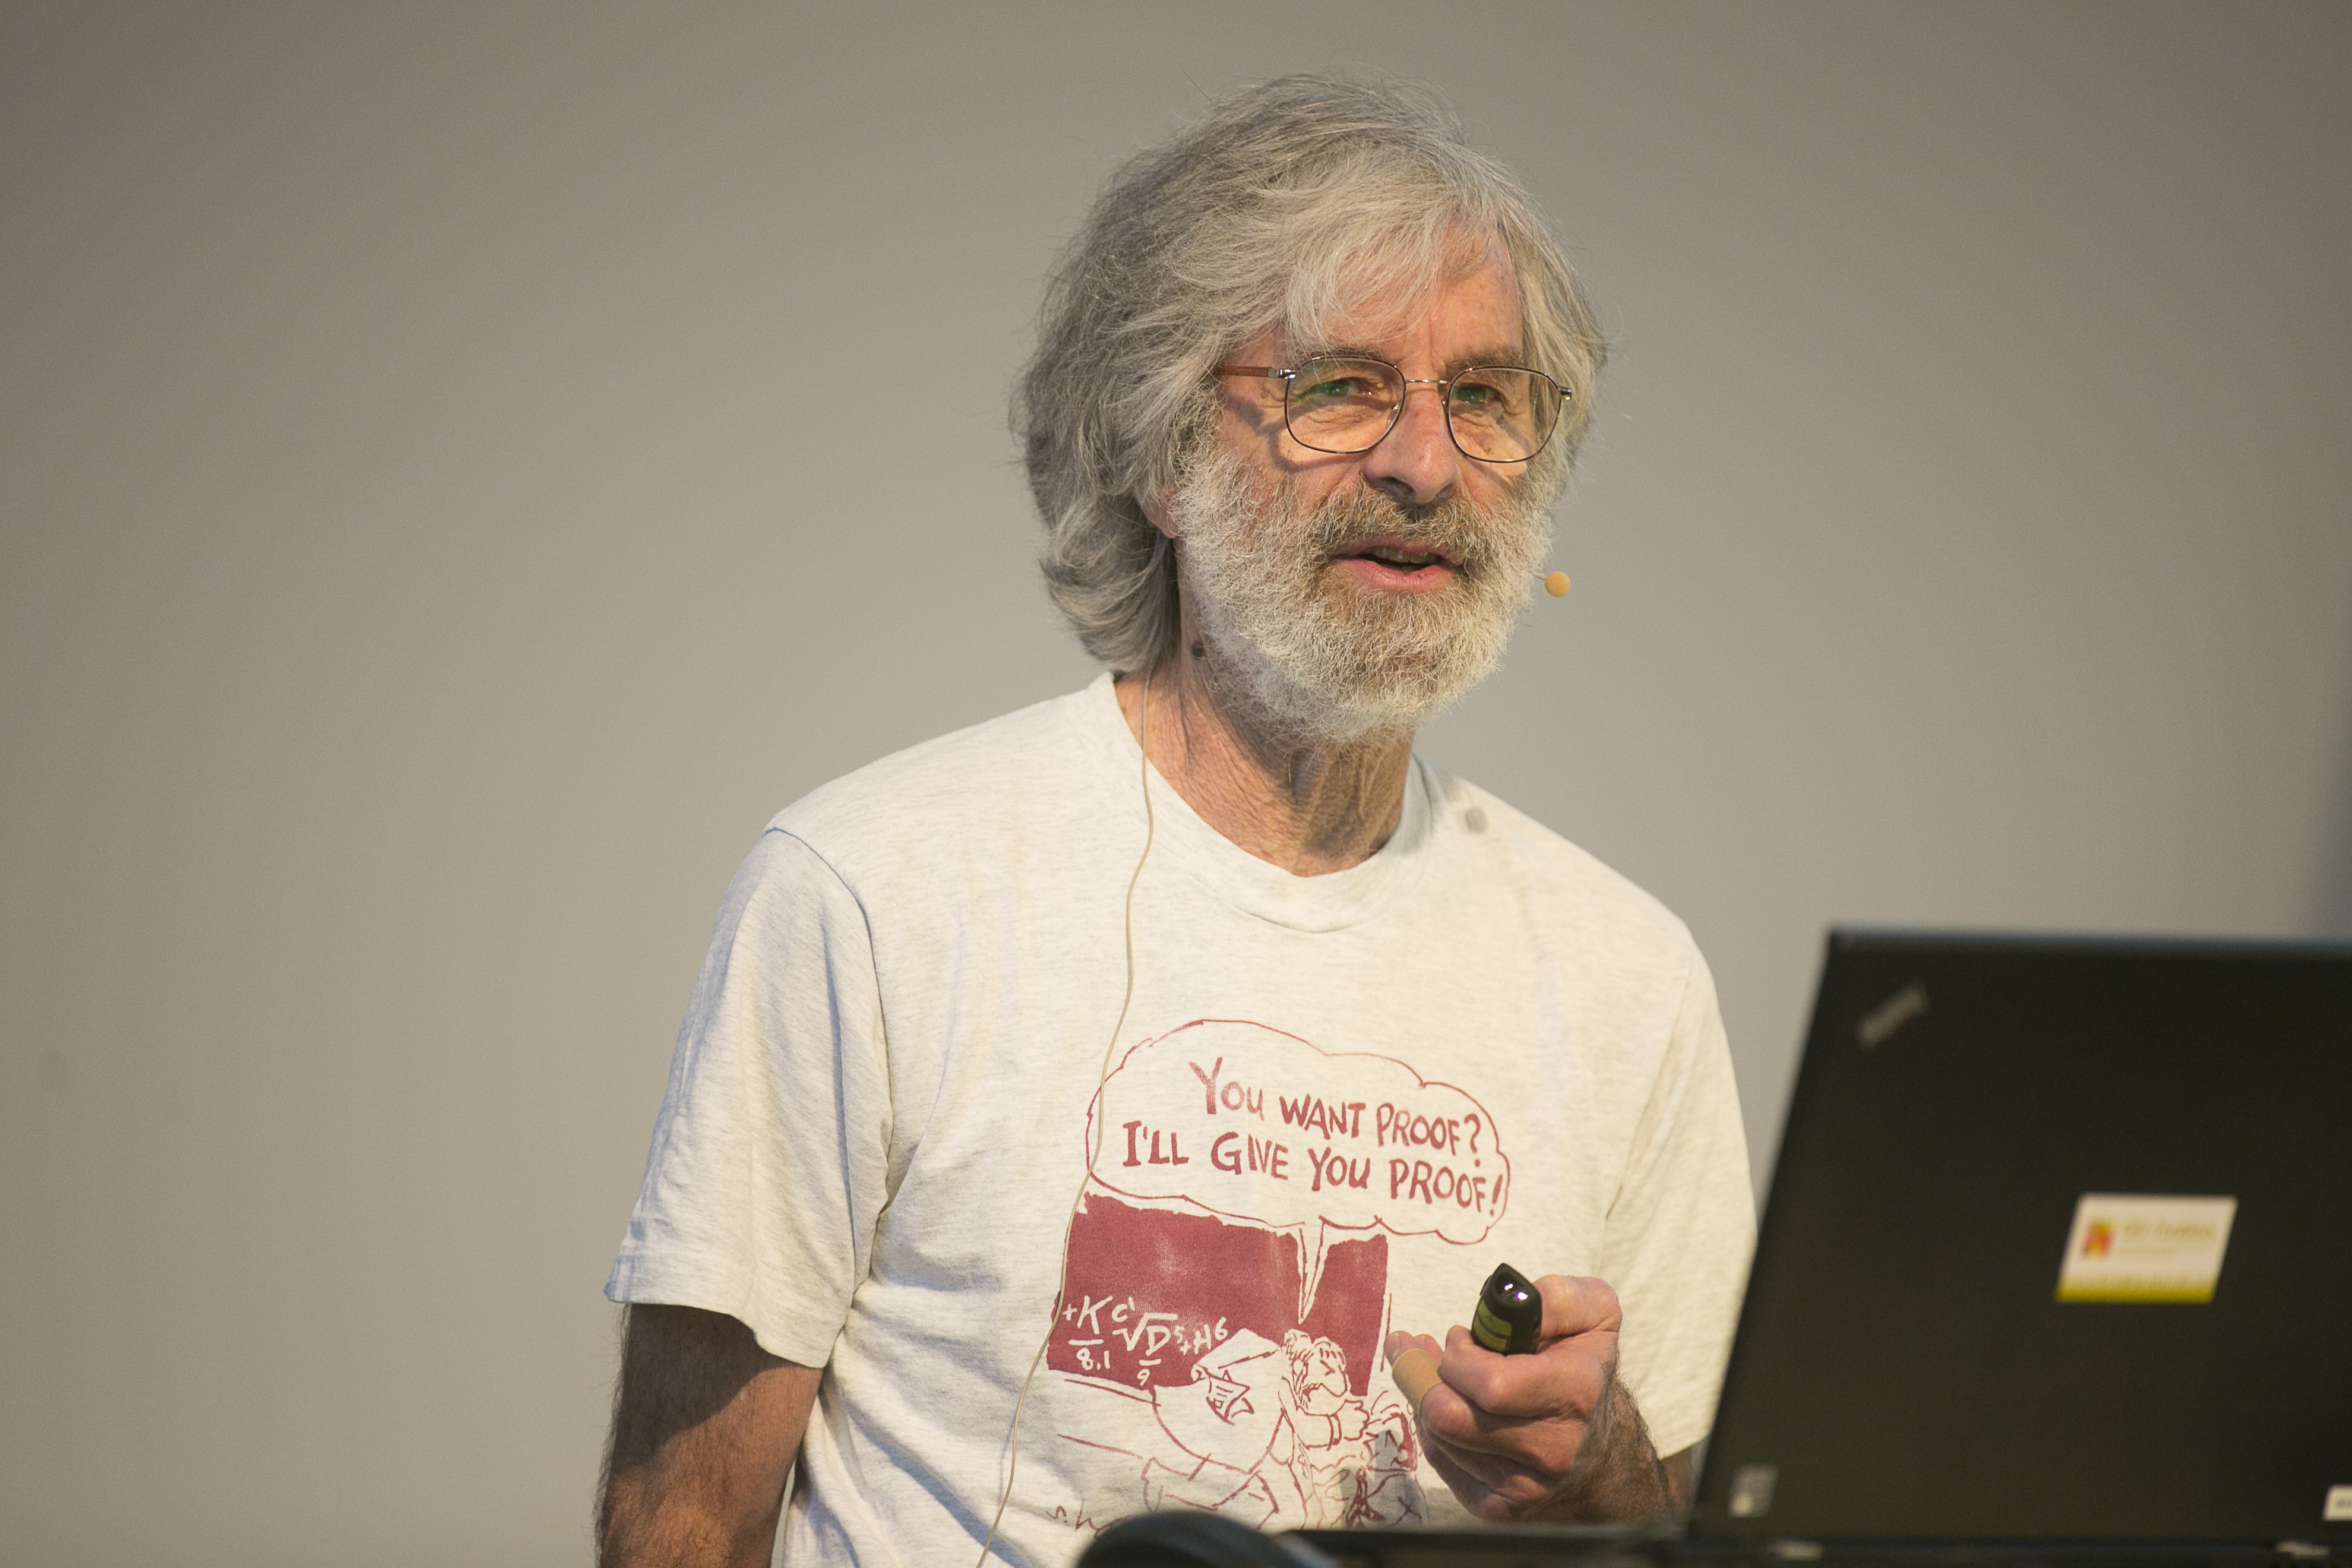
\includegraphics[width=10cm]{images/Lamport-Kreutzer}
\end{center}

\end{frame}

\begin{frame}[fragile]
\frametitle{\textbf{?`Qué es \LaTeX{}?}}
\justifying
 \begin{itemize}\justifying
  \item Su proposito es simplificar el manejo de \TeX{}.
  \item \LaTeX{} permite que los autores impriman sus documentos con la mayor calidad tipográfica usando formatos predefinidos y profesionales.
  \item Usa \TeX{} como motor tipografiado.
  \item Es especialmente adecuado para documentos que contengan expresiones matemáticas.
  \item Es un editor del tipo WYSIWYM (What You See is What You Mean). Se basa en un lenguaje de marcado como el HTML o el lenguaje wiki.
\end{itemize}

\end{frame}

\section{Ventajas e Inconvenientes}
\subsection{Desventajas de \LaTeX{}}
 \begin{frame}[fragile]
\frametitle{\textbf{Desventajas}}
\justifying
\begin{block}{Resultado del documento}
\begin{itemize}\justifying
  \item No se ve el resultado final mientras se edita el documento.
  \begin{itemize}\justifying
  \item Eso ayuda a no distraerse...
  \item pero conviene compilar de vez en cuando para ver cómo está quedando y evitar acumulación de errores.
\end{itemize}

\end{itemize}
	
\end{block}
\begin{block}{Curva de Aprendizaje}
\begin{itemize}\justifying
  \item Hay que aprender una colección de comandos.
  \begin{itemize}\justifying
  \item No hay que aprender todos los comandos de \LaTeX{}.
  \item Se aprenden los comandos básicos y los que se vayan necesitando.
  \item Podemos partir de una plantilla e ir mirando los comandos, en lugar de escribir desde 0.
\end{itemize}
\end{itemize}
\end{block}
\end{frame}

\begin{frame}[fragile]
\frametitle{\textbf{Desventajas}}
\justifying
 \begin{block}{Errores de Compilación}
\begin{itemize}\justifying
  \item Se pueden producir errores de compilación.
  \begin{itemize}\justifying
  \item Ir compilando con frecuencia.
  \item Cortar o comentar partes del código para localizar el problema.
\end{itemize}

\end{itemize}

\end{block}

\begin{block}{Personalización}
\begin{itemize}\justifying
  \item Es complicado conseguir un \textit{look} o \textit{layout} concreto.
  \begin{itemize}\justifying
  \item No es una herramienta de diseño, el proceso es incómodo.
  \item Una vez creado el \textit{layout} deseado, sí es muy fácil utilizarlo en nuevos documentos.
  \item Generalmente, los editores diseñan la plantilla, los autores simplemente la rellenan.
\end{itemize}

\end{itemize}

\end{block}

\end{frame}
\subsection{Ventajas de \LaTeX{}}
\begin{frame}[fragile]
\frametitle{\textbf{Ventajas}}
\justifying
 \begin{block}{Separación de contenido y formato}
\begin{itemize}\justifying
  \item Abstracción entre presentación y contenido.
  \begin{itemize}\justifying
  \item El autor se centra en la estructura del documento.
  \item Elimina muchas pérdidas de tiempo dedicadas a la presentación del documento.
  \item El formato lo asigna un maquetador profesional (\LaTeX{}).
\end{itemize}

\end{itemize}

\end{block}

\begin{block}{Disponibilidad de Plantillas}
\begin{itemize}\justifying
  \item Disponibilidad de plantillas profesionales.
  \begin{itemize}\justifying
  \item El escritor no tiene que diseñar una plantilla adecuada, ya existen muchas.
  \item Plantillas por defecto en \LaTeX{} (book, article, letter, etc).
  \item Plantillas creadas por otras personas: IEEE, universidades, ltsas...
\end{itemize}

\end{itemize}

\end{block}
\end{frame}

\begin{frame}[fragile]
\frametitle{\textbf{Ventajas}}
\justifying
 \begin{block}{Fórmulas}
\begin{itemize}\justifying
  \item Introducción de fórmulas complejas de forma cómoda.
  \item Ejemplo:
  \begin{itemize}\justifying
  \item $\Delta v = \frac{v_o}{v_i} = \frac{v_b}{v_c} = \frac{1V}{10mV} = 100$
  \item \verb+$\Delta v = \frac{v_o}{v_i} = \frac{v_b}{v_c} = +\\\verb+\frac{1V}{10mV} = 100$+
\end{itemize}

\end{itemize}

\end{block}

\begin{block}{Generación automática de estructuras complejas}
\begin{itemize}\justifying
  \item Permite generar estructuras complejas de forma sencilla:
  \begin{itemize}\justifying
  \item Índices (de contenido, de tablas, de figuras)
  \item Referencias cruzadas (entre capítulos, tablas, etc.)
  \item Bibliografía.
\end{itemize}

\end{itemize}

\end{block}


\end{frame}


\begin{frame}[fragile]
\frametitle{\textbf{Ventajas}}
\justifying
 \begin{block}{Software Libre, muy estable y portable}
\begin{itemize}\justifying
  \item Software libre: disponibilidad de muchos paquetes e información de la comunidad. Software Gratuito.
  \item Sistema muy estable, virtualmente libre de bugs.
  \item Muy portable.
  \begin{itemize}\justifying
  \item Se puede utilizar en diferentes equipos y sistemas operativos.
\end{itemize}

\end{itemize}

\end{block}
\begin{block}{Lenguaje Estándar}
\begin{itemize}\justifying
  \item Lenguaje estándar: se ve igual en cualquier equipo, y seguirá siendo así con el paso de los años (se evita el problema de versiones de los procesadores de textos).
  \item Muy extendido en el mundo académico.
  \item Estándar de facto para la publicación en revistas muy prestigiosas: IEEE, ACM, etc.
\end{itemize}

\end{block}

\end{frame}

\begin{frame}[fragile]
\frametitle{\textbf{Ventajas}}
\justifying
 \begin{block}{Resultados tipográficos}
\begin{itemize}\justifying
  \item Resultados tipográficos de calidad profesional.
  \item \LaTeX{} se encarga de maquetar nuestro texto de forma profesional.
  \item Soporte para diferentes tipografías.
\end{itemize}

\end{block}
\begin{block}{Independencia del formato}
\begin{itemize}\justifying
  \item Facilidad para cambiar entre formatos de documentos.
  \item Podemos escribir un artículo y ampliarlo hasta convertirlo en un libro.
  \item Para que el formato se adapte solo hay que indicarle a \LaTeX{} que ahora queremos un formato de libro.
\end{itemize}

\end{block}

\end{frame}

\begin{frame}[fragile]
\frametitle{\textbf{Ventajas}}
\justifying
 \begin{block}{Archivos en texto plano}
\begin{itemize}\justifying
  \item Requiere pocos recursos de la máquina.
  \item Ocupa poco espacio, ventaja para enviar por email.
  \item Formato adecuado para trabajar con sistemas de control de versiones.
  \item Facilidad para la generación de documentos a partir de scripts.
\end{itemize}

\end{block}

\begin{block}{Comandos}
La posibilidad de escribir nuestros propios comandos (o añadir comandos que otros han escrito).
\end{block}


\end{frame}

\section{Principio de Funcionamiento}
\begin{frame}[fragile]
\frametitle{\textbf{Principio de Funcionamiento}}
\justifying
 \begin{enumerate}\justifying
  \item El usuario escribe el contenido estructurado mediante el lenguaje de marcado.
  \item Se compila, y \LaTeX{} formatea el texto en líneas, párrafos y páginas, asignando el formato adecuado (numeración, tipos de letra, etc).
  \item Se visualiza en pantalla el documento de salida.
  \item Se vuelve al punto 1 hasta conseguir el resultado final deseado.
\end{enumerate}

\end{frame}

\begin{frame}[fragile]
\frametitle{\textbf{Procesadores Tradicionales VS \LaTeX{}}}
\justifying
\begin{center}
 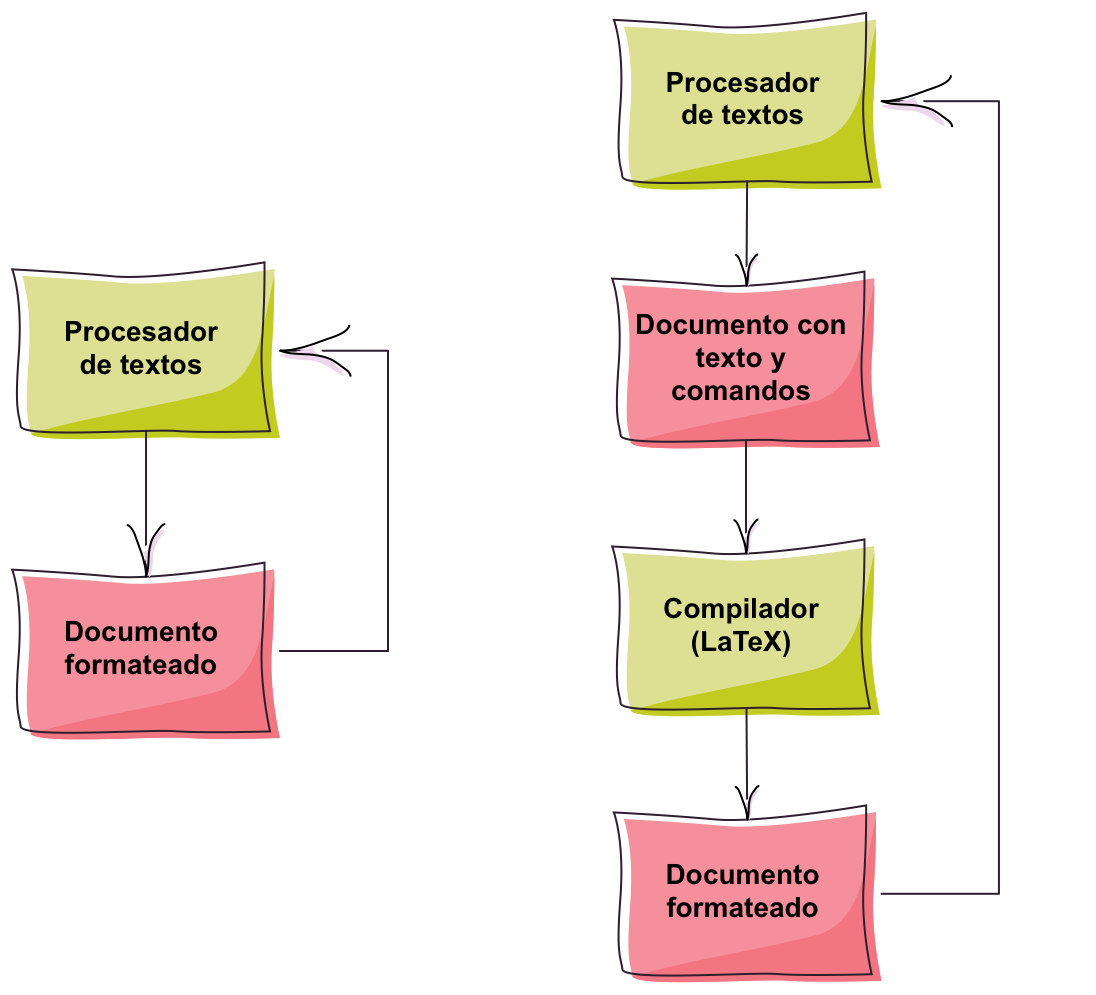
\includegraphics[width=8.5cm]{images/vs}
\end{center}

\end{frame}
\subsection{structura del documento}
\begin{frame}[fragile]
\frametitle{\textbf{Estructura del documento}}
\justifying
 \begin{itemize}\justifying
  \item Se crea una carpeta que contendrá el documento con un nombre identificativo.
  \item Dentro de la carpeta, se creará un archivo con el contenido, con extensión .tex.
  \item Crear también un directorio donde se guardarán las imágenes dentro de la carpeta del documento. Ej: images.
  \item No utilizar tildes ni espacios en los nombre de los archivos ni de documentos.
  \item Al compilar, se generan archivos adicionales.
\end{itemize}

\end{frame}

\begin{frame}[fragile]
\frametitle{\textbf{Archivos generados al compilar}}
\justifying
 \begin{itemize}\justifying
  \item [.log] Registro detallado de qué pasó durante la compilación.
  \item [.toc] Almacena las cabeceras de sección. Se lee en la siguiente compilación para producir el índice.
  \item [.lof] Como .toc pero para la lista de figuras.
  \item [.lot] Lo mismo, pero para tablas.
  \item [.aux] Entre otras cosas, se usa para las referencias cruzadas.
  \item [.idx] Almacena las palabras del índice alfabético, si se está usando.
  \item [.ind] Contiene información del índice alfabético cuando .idx es procesado.
  \item [.ilg] Registro de lo que hizo .ilg.
\end{itemize}

\end{frame}

\subsection{Concepto de Paquete}
\begin{frame}[fragile]
\frametitle{\textbf{Concepto de Paquete}}
\justifying
 \begin{itemize}\justifying
  \item Los paquetes son piezas de software que proporcionan funcionalidades adicionales.
  \item Hay muchos paquetes instalados por defecto. Se puede indicar que los vamos a usar con \verb+\usepackage+.
  \item Para usar paquetes que no vienen por defecto, primero hay que instalarlos (ya veremos cómo).
\end{itemize}

\end{frame}

\subsection{Programas Requeridos}
\begin{frame}[fragile]
\frametitle{\textbf{Programas Requeridos}}
\justifying
 \begin{block}{Programas Necesarios}
\begin{itemize}\justifying
  \item Editor de texto plano.
  \item Compiladores \LaTeX{}.
  \item Visores para los diferentes formatos (.dvi, .ps, .pdf, .png)
\end{itemize}

\end{block}
\end{frame}


\begin{frame}[fragile]
\frametitle{\textbf{Compiladores}}
\justifying
 \begin{block}{Compiladores \LaTeX{}}
\begin{description}\justifying
  \item [GNU/Linux] \TeX{}-live (en repositorios)
  \item \begin{itemize}\justifying\scriptsize
  \item[] Instalar los siguientes paquetes: preview-latex-style texlive-full texlive texlive-latex-extra texlive-math-extra texlive-pstricks texlive-science latex-beamer aspell aspell-es latexila
\end{itemize}

  \item [MacOSX] Mac\TeX{} (http://www.tug.org/mactex)
  \item [Windows] MiK\TeX{} (http://miktex.org)
  \begin{itemize}\justifying\scriptsize
  \item[] En el menú Downloads, seleccionar la versión, descargar y guardarlo en el directorio deseado y luego ejecutar.
\end{itemize}

\end{description}

\end{block}

\end{frame}


\begin{frame}[fragile]
\frametitle{\textbf{Compiladores}}
\justifying
 \begin{block}{Función del Compilador}
\begin{itemize}\justifying
  \item El compilador es necesario para interpretar el archivo de texto plano con el lenguaje de marcado y maquetarlo.
  \item En GNU/Linux, al instalar un editor como Kile, los compiladores se instalan automáticamente.
\end{itemize}

\end{block}

\end{frame}

\begin{frame}[fragile]
\frametitle{\textbf{Compiladores}}
\justifying
 \vspace{-0.5cm}
 \begin{center}
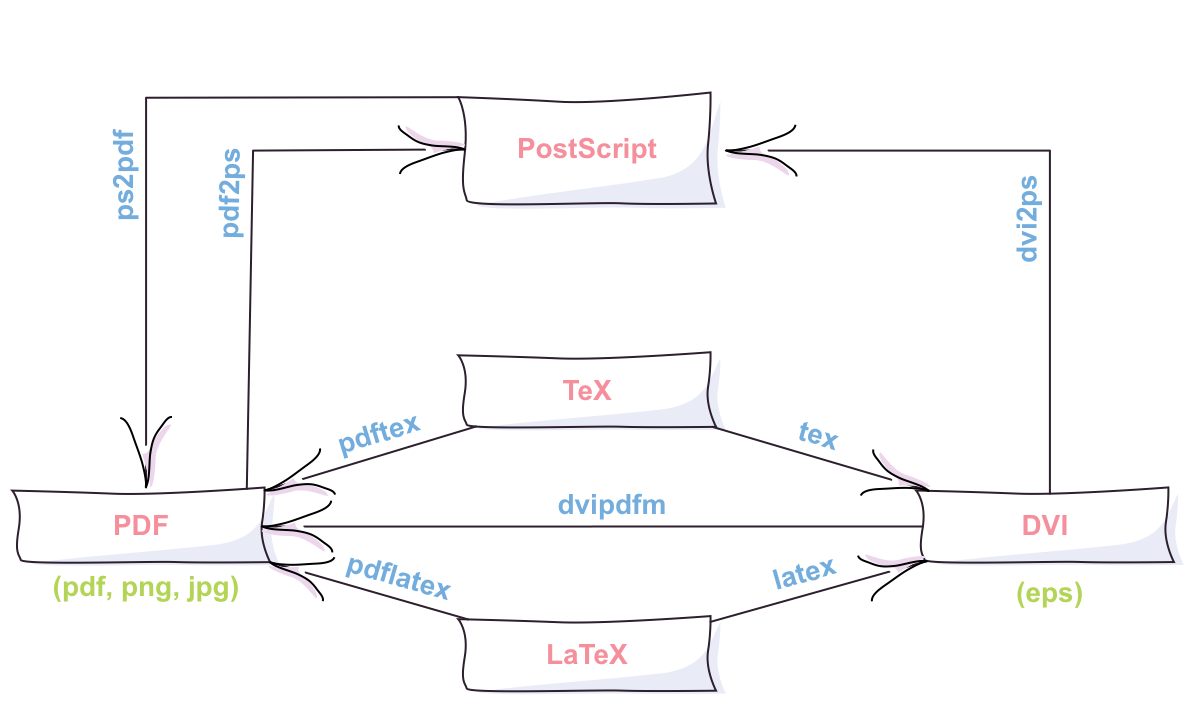
\includegraphics[width=11cm]{images/compiador}
\end{center}
\vspace{-0.5cm}
 \begin{itemize}\justifying
  \item \textbf{Rojo}: Formatos de documento.
  \item \textbf{Azul}: Compiladores y conversores de formato.
  \item \textbf{Verde}: Formatos gráficos soportados por cada compilador.
\end{itemize}

\end{frame}

\begin{frame}[fragile]
\frametitle{\textbf{Programas Requeridos}}
\justifying
 Los formatos soportados dependen del compilador:
 \begin{itemize}\justifying
  \item \verb+$ latex archivo.tex+ $\rightarrow$ archivos *.eps
  \item \verb+$ pdflatex archivo.tex+ $\rightarrow$ archivos *.pdf *.ps *.jpg *.png
\end{itemize}
Las imagenes *.eps son del tipo vectorial.
\begin{block}{Formato de documento e imagen}
\begin{itemize}\justifying
  \item ?`Con qué formatos de documentos suelen trabajar? *.pdf, *.ps, etc.
  \item ?`Con qué formatos de imágen? *.png, *.eps, *.jpg
\end{itemize}

\end{block}

\end{frame}

\begin{frame}[fragile]
\frametitle{\textbf{Editores de Texto Plano}}
\justifying
 \begin{block}{Editores Básicos}
Vim, nano, pico, emacs, notepad++, notepad, greany, chocolate, sublime text, etc.
\end{block}

\begin{block}{Editores Especializados}
Kile, \TeX{}nicCenter, \TeX{}MakerX, WinEdt, \TeX{}Pad, Gummy, \LaTeX{}ila, etc.
\end{block}


\begin{block}{Editores Online}
\begin{itemize}\justifying
  \item \href{https://www.sharelatex.com?r=3e23a01e&rm=d&rs=b}{\textbf{Share\LaTeX{}}}
  \item \href{https://www.overleaf.com/signup?ref=f53152975118}{\textbf{Overleaf}}
\end{itemize}

\end{block}
\end{frame}

\begin{frame}[fragile]
\frametitle{\textbf{Recomendación}}
\justifying
 \begin{block}{Linux}
Gummy y/o \LaTeX{}ila
\begin{itemize}\justifying
  \item Software Libre y Gratuito
  \item Disponible en los repositorios
  \item Resaltado de Sintaxis
  \item Visualización de avance (Gummy)
  \item Corrector Ortográfico (hay que configurarlo)
  \item Selector de símbolos matemáticos y etiquetas (\LaTeX{}ila)
\end{itemize}
\end{block}
\end{frame}


\begin{frame}[fragile]
\frametitle{\textbf{Recomendación}}
\justifying

\begin{block}{Windows}
\TeX{}MakerX
\begin{itemize}\justifying
  \item Software Libre y Gratuito
  \item Multiplataforma
  \item Versión Portable
  \item Resaltado de Sintaxis
  \item Corrector Ortográfico (hay que configurarlo)
  \item Selector de símbolos matemáticos y etiquetas
  \item Referencia de sintaxis de \LaTeX{}
\end{itemize}

\end{block}
\end{frame}

\begin{frame}[fragile]
\frametitle{\textbf{Instalar \LaTeX{}}}
\justifying
\begin{block}{En Linux}
 \begin{itemize}\justifying
  \item Instalar los paquetes: \textbf{preview-latex-style texlive-full texlive texlive-latex-extra texlive-math-extra texlive-pstricks texlive-science latex-beamer aspell aspell-es latexila gummy}
\end{itemize}
\end{block}
\end{frame}


\begin{frame}[fragile]
\frametitle{\textbf{Visores de Documentos}}
\justifying
 
 \begin{itemize}\justifying
  \item Visores para *.pdf, *.dvi y *.ps en función del formato que usemos.
  \item Portable Windows:
  \begin{itemize}\justifying
  \item [.dvi]: visor Yap contenido en MiK\TeX{}\footnote{\url{http://miktex.org/portable}}
  \item [.ps]: Instalar Ghostcript\footnote{\url{http://www.ghostscript.com}} y Gsview\footnote{\url{http://pages.cs.wisc.edu/~ghost/gsview/index.htm}}
  \item [.pdf]: Cualquier visor pdf: Sumatra PDF\footnote{\url{http://www.sumatrapdfreader.org/free-pdf-reader-es.html}} (libre), Acrobat Reader, Foxit Reader\footnote{\url{http://portableapps.com/apps/office/foxit_reader_portable}}
\end{itemize}
\end{itemize}
\begin{block}{Visores PDF}
\begin{itemize}\justifying
  \item Acrobat Reader o Foxit Reader Sirven:
  \begin{itemize}\justifying
  \item Pero requieren cerrar el documento antes de volver a compilar.
  \item Eso suele resultar molesto.
\end{itemize}

  \item Sumatra PDF:
  \begin{itemize}\justifying
  \item Libre, gratuito, y no hace falta cerrar el documento.
  \item Se abre el pdf una vez y cada vez que se compila se actualiza.
\end{itemize}

\end{itemize}

\end{block}

 
\end{frame}





\end{document}